\section{Sprint 7} % DROPBOX

\subsection{Planificación}
\begin{itemize}
    \item \textbf{Inicio}: 1 de octubre del 2015.
    \item \textbf{Fin}: 17 de octubre del 2015.
\end{itemize}


\subsection{Descripción}

En este sprint se busca brindarle al usuario la funcionalidad para poder gestionar imágenes. Son varios los casos en los que una persona concurre a una institución médico, realiza una serie de estudios como consecuencia de la consulta y obtiene resultados en forma de papel impreso o imágenes. Con la funcionalidad desarrollada en este sprint, el usuario puede tomar una imagen del documento o el archivo de la imagen tomada en el estudio, crear un análisis en yesdoc y adjuntar al análisis dichas imágenes. Podemos decir entonces que este análisis mantiene un respaldo digital de lo que es una consulta y de los documentos documentos resultantes de la misma, un análisis clínico, una imagen de radiografía y demás documentos médicos físicos. Para cumplir con esta funcionalidad el equipo tuvo que definir un medio de almacenamiento, para esto se eligió la nube. Existen muchos y variados medios de almacenamiento en la nube como son Dropbox, Drive, Mega, entre otros. Teniendo en cuenta esta situación, el equipo tuvo que definir una forma de conectarse con los mismos adaptando la comunicación de acuerdo a cada una en particular y reduciendo el impacto frente al cambio siempre teniendo en cuenta la alta cohesión y el bajo acoplamiento.
	
	
	Este sprint le permite al usuario:
	\begin{itemize}
		\item Elegir el medio de almacenamiento en la nube de preferencia y, en caso de que no cuente con uno, utilizar el que YesDoc ofrece por defecto.
		\item Brindar un flujo de autorización, por parte del usuario para que YesDoc use el almacenamiento seleccionado, integrado en el sistema y intuitivo.
		\item Cargar, descargar y eliminar imágenes en un análisis.
		\item Listar las imágenes de un análisis.
		\item Cambiar el medio de almacenamiento seleccionado cuando lo desee. % consultar si está implementado			
	\end{itemize}
	  


\subsection{Sprint backlog}


{\scriptsize
	\begin{center} %sidewaystable
		\centering
		%\begin{adjustbox}{max width=\textheight}
		\resizebox{\textwidth}{!}{
			\begin{tabular}{|l|l|l|p{6cm}|l|l|}
				\hline
				\textbf{Area a cargo} &
				\textbf{Responsable} &  
             	\textbf{Revisor} &       
				\textbf{Tarea} &
				\textbf{US} &
				\textbf{tiempo dedicado}\\ 
				\hline
				Back-end& Franco Canizo & Michael Manganiello & Se define la estructura para la gestión de archivos & US-\ref{resumenInfo} \& US-\ref{infoSalud} & 4hs \\ 
				\hline
				Back-end& Franco Canizo& Michael Manganiello & Se crea el adaptador para la gestión de archivos en dropbox , se crea el recurso para la carga y descarga de archivos de análisis. & US-\ref{resumenInfo} \& US-\ref{infoSalud} & 24hs \\ 
				\hline
				Back-end& Michael Manganiello & todos& Se añaden las clases del dominio y funcionalidades para el manejo de análisis, archivos asociados, y la gestión de credenciales a diferentes servicios de almacenamiento personales del usuario & US-\ref{resumenInfo} \& US-\ref{infoSalud} & 6hs \\ 
				\hline
				Back-end& Michael Manganiello &Franco Canizo & Creación de la migración para los nuevos modelos & US-\ref{resumenInfo} \& US-\ref{infoSalud} & 2hs \\ 
				\hline
				Back-end& Michael Manganiello &Franco Canizo & Creación de fields y parsers para las representaciones de los nuevos recursos & US-\ref{resumenInfo} \& US-\ref{infoSalud} & 2hs\\ \hline
				Back-end& Michael Manganiello & Franco Canizo & Correcciones generales de integración, claves de la aplicación en Dropbox, devolución y eliminación de archivos & US-\ref{resumenInfo} \& US-\ref{infoSalud} & 16hs\\ 
				\hline
			\end{tabular}
		}
		%\end{adjustbox}
	\end{center}
}

\subsection{User Stories relacionados}
La \textbf{Tabla \ref{US-Sprint6} } indicará las características de cada user story para guiarnos en el desarrollo del sprint.

\begin{table}[h]
    \label{US-Sprint7}
	%\resizebox{\textwidth}{!}{
    \centering
	\begin{tabular}{|l|p{9cm}|}
	\hline
        \multicolumn{1}{|c|}{\textbf{ID}} &
        \multicolumn{1}{|c|}{\textbf{Enunciado de la historia}} \\          
    \hline
        \textbf{US-1 } & Como paciente, quiero  añadir información de mi perfil de salud o mediciones regulares para que el médico cuente con más y mejor información al momento de realizar el diagnóstico. \\
    \hline
        \textbf{US-2 } & Como paciente, quiero añadir al sistema los estudios realizados para evitar posibles perdidas.\\
     \hline
        \textbf{US-16 } & Como paciente, quiero acceder a mis documentos desde cualquier lugar para hacer uso de ellos cuando los necesite.\\
     \hline   
     
    \end{tabular}
%     }
\end{table}

\subsection{Modelo funcional} 
Se describirán las funciones usando como marco de apoyo el sprint Backlog, además se armará el diagrama de casos de uso del presente Sprint \textbf{[Figura \ref{6-cu_file_upload}]} que irá creciendo  medida se vaya avanzando en el proyecto.

    \begin{figure}[h]
        \centering
        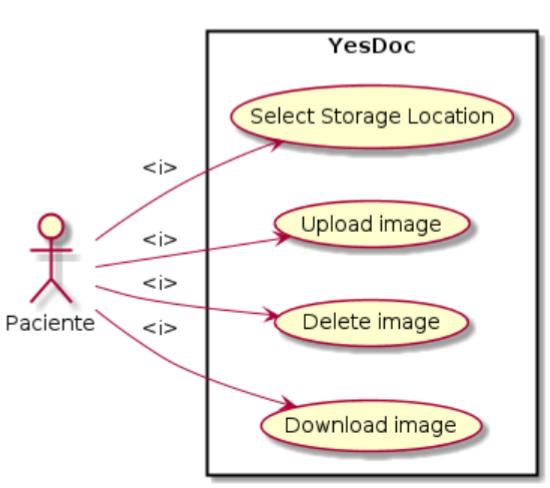
\includegraphics[width=0.5\textwidth]{img/cu_file_upload}
        \caption{CU-Gestión de archivos}
		\label{6-cu_file_upload}
    \end{figure}
    
\newpage

\subsection{Modelo de datos}
El Diagrama propio de este sprint se puede ver en la \textbf{Figura \ref{6-clases_file_upload}}, allí se indican exactamente las clases que se usarán en este sprint y que serán detalladas con detenimiento en el presente documento. Se recuerda que se ha realizado un Diagrama de clases específico para este sprint y puede variar en futuras iteraciones.
% Se fue a la mierda esta imágen
    \begin{figure}[h]
        \centering
        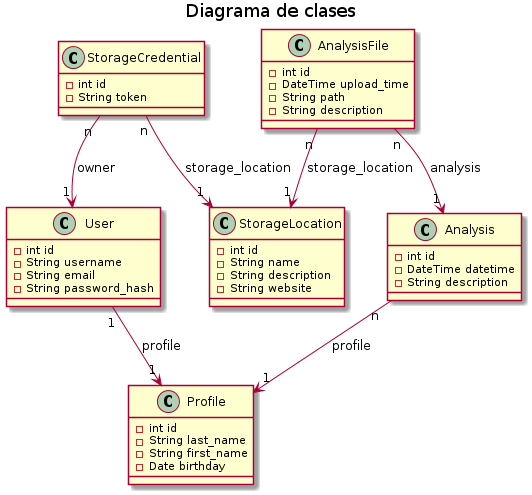
\includegraphics[width=0.5\textwidth]{img/dc_file_upload}
        \caption{Clases para la gestión de archivos.}
		\label{6-clases_file_upload}
    \end{figure}


\subsection{Diseño} 

\subsubsection{Estructura conexión con diferentes medios de almacenamiento}
	Se define el paquete ``adapters'' en el cual se define una fábrica encargada de la creación del adaptador específico para la conexión y gestión de archivos con el medio de almacenamiento específico. Para la situación actual del sistema se definen dos adaptadores específicos, uno para el almacenamiento por defecto en la cuenta de YesDoc y otro para el almacenamiento de archivos en Dropbox. La \textbf{Figura \ref{6-dcd_file_upload}} muestra el diagrama de clases de diseño específico.

	\begin{figure}[h]
        \centering
        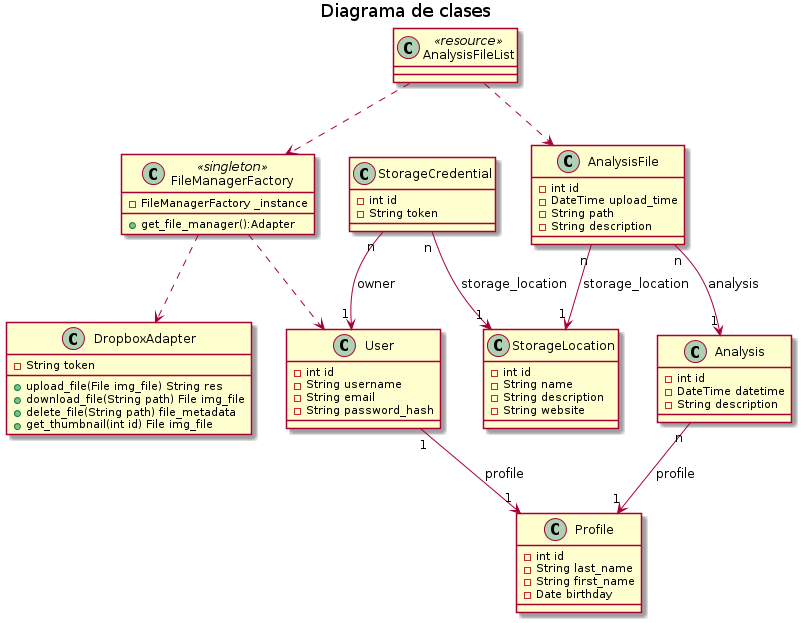
\includegraphics[width=0.9\textwidth]{img/dcd_file_upload}
        \caption{DCD-Carga de archivos}
		\label{6-dcd_file_upload}
    \end{figure}
   
\newpage

	En este diseño se aplicaron los patrones:
		\begin{itemize}			
			\item Alta cohesión.
			\item Bajo acoplamiento.
			\item Singleton
			\item Factoría
			\item Adaptador
		\end{itemize}

\subsubsection{Modelos para la gestión de archivos}

Se crean las clases del modelo lógico que definimos en la \textbf{Figura \ref{6-clases_file_upload}}, de cada una de estas se definen los atributos siguiendo la documentación de SQLAlchemy, ORM utilizado para mapeo de las entidades de la API, sus relaciones y funcionalidades. 

El modelo \textbf{StorageCredential} guarda el token que recibe la API luego de que el usuario autorice a la aplicación a usar su almacenamiento en dropbox para gestionar archivos. Cada StorageCredential mantiene una relación con User y StorageCredential.

El modelo \textbf{StorageLocation} mantiene un identificador y datos generales del medio de almacenamiento de preferencia del usuario a partir de los ofrecidos por la API.

El modelo \textbf{AnalysisFile} mantiene datos relacionados con la gestión del archivo como la ruta, nombre, fecha de carga y está relacionado con el modelo Analysis y StorageLocation lo que nos permite asignar varios archivos a un análisis, archivos que pueden estar almacenados en distintos medios de almacenamiento en la nube.

\subsubsection{Creación de la migración para los nuevos modelos}

Una vez definidas las clases se obtiene a partir de migrate un script sql con la nueva versión de la base de datos, script que utilizamos para actualizar las tablas de la base de datos para incorporar las nuevas a partir de los modelos previamente definidos. Esto es posible gracias al uso de las extensiones \textbf{flask-migrate} para las migraciones de la base de datos y \textbf{flask-script} para la ejecución de comandos externos.

\subsubsection{Definición de Recursos}

Para que el cliente se comunique con los modelos que hemos definido la API define recursos encargadas de manejar estos modelos:

El recurso \textbf{AnalysisAnalysisFileList} permite la obtención de los archivos asociados a un análisis específico. El usuario debe estar autenticado. El servicio se brinda a través del método GET.

\textbf{AnalysisFileDownload} permite la descarga de un archivo específico desde el medio de almacenamiento en la nube. Requiere autenticación. El servicio se brinda a través del método GET.

\textbf{AnalysisFileThumbnail} permite obtener la vista previa de un archivo específico. Requiere autenticación. El servicio se brinda a través del método GET.

\textbf{AnalysisFileView} permite obtener, a través del servicio GET, datos cargados en el modelo AnalysisFile, por medio de PUT se  puede modificar los datos almacenados de un archivo y DELETE para eliminar los datos y el archivo correspondiente en la nube. Todos estos servicios mencionados requieren previa autenticación.

El método auxiliar delete\_file en el archivo \textbf{analysisFile} en el directorio ``persistence'' elimina un archivo del medio de almacenamiento en la nube.

\textbf{AnalysisFileList} brinda servicio GET para obtener todas las instancias de AnalysisFile correspondientes a los archivos cargados a YesDoc y, a través del servicio POST, cargar un nuevo AnalysisFile y el archivo al medio de almacenamiento de preferencia para el usuario. El servicio POST requiere autenticación.

\textbf{StorageCredentialView} brinda los servicios GET para obtener una instancia específica de credencial y PUT para actualizar una instancia específica de StorageCredential.

\textbf{StorageCredentialList} brinda los servicios GET para obtener las credenciales de almacenamiento cargadas y POST para cargar una nueva credencial de almacenamiento.

\textbf{StorageLocationView} brinda los servicios GET para obtener una instancia específica de ubicación de almacenamiento y PUT para actualizar una instancia específica de ubicación de almacenamiento.	

\textbf{StorageLocationList} brinda los servicios GET para obtener todas las ubicaciones de almacenamiento cargadas y POST para cargar una nueva ubicación de almacenamiento.

\textbf{MyStorageCredentialList} por medio del servicio GET retorna todas las instancias existentes de credencial de almacenamiento, asociadas al usuario autenticado. A través del servicio POST crea una nueva instancia de credencial de almacenamiento asociada al usuario autenticado, y la retorna.

Se añade al recurso \textbf{AnalysisView} el servicio DELETE para eliminar todas las imágenes asociadas a un análisis específico. Elimina también el análisis. Requiere que el usuario esté autenticado.

\subsubsection{Identificadores(URI)}
Para acceder a estos recurso el equipo pone a disposición del cliente los siguientes identificadores:

\begin{itemize}
	\item\textbf{/analysis/<int:analysis\_id>/files}
	\item\textbf{/analysis/<int:analysis\_id>}
	\item\textbf{/analysis\_files/<int:id>/download}
	\item\textbf{/analysis\_files/<int:analysis\_file\_id>/thumbnail}
	\item\textbf{/analysis\_files/<int:id>}
	\item\textbf{/analysis\_files}
	\item\textbf{/storage\_credentials/<int:id>}
	\item\textbf{/storage\_credentials}
	\item\textbf{/storage\_locations/<int:id>}
	\item\textbf{/storage\_locations}
	\item\textbf{/my/storage\_credentials}
\end{itemize}

\subsubsection{Representaciones}
Finalmente se arman las representaciones que el cliente debe tener en cuenta al momento de enviar y recibir datos. Las definiciones bajo el directorio ``parsers'' determinan la representación para las solicitudes HTTP del cliente al servidor mientras que las definidas bajo el directorio ``fields'' definen la representación para las respuestas del servidor al cliente.





\subsection {Salidas del Sistema - Incrementos}
\textbf{Carga de una credencial de almacenamiento}

Para la carga debemos utilizar el recurso que la API presenta con el identificador único URL \textbf{\/storage\_credentials}. Suponemos que previamente el usuario de prueba ha autorizado a nuestra aplicación a que utilice espacio del almacenamiento de su cuenta de dropbox y por lo tanto contamos con el token: ``Jl0\_uroqYBoAAAAAAAA
F6KUxPAlgAMTqFf9ES2S0zZl\_27V5QAmEn5V58IUxcck1''. Suponemos que ha sido cargado en API un usuario con id 1 y un storage location con id 2. Teniendo en cuenta la representación definida para la solicitud al recurso y que debemos usar el método POST para cargar la credencial, ejecutamos la siguiente linea CURL:

\begin{verbatim}
curl -i http://localhost:5000/storage_credentials -H "Content-Type: 
application/json" -X POST -d '{"token":"Jl0_uroqYBoAAAAAAAAF6KUxPAl
gAMTqFf9ES2S0zZl_27V5QAmEn5V58IUxcck1", "owner_id":"1", 
"storage_location_id":"1"}'
\end{verbatim}

La API nos responde con la siguiente respuesta:

\begin{lstlisting}[language=json]
HTTP/1.0 201 CREATED
Content-Type: application/json
Content-Length: 812
Server: Werkzeug/0.10.4 Python/2.7.6
Date: Tue, 20 Oct 2015 19:10:33 GMT

{
    "resource": {
        "id": 2, 
        "owner": {
            "email": "fncanizo@gmail.com", 
            "id": 1, 
            "profile": {
                "birthday": "1990-06-20", 
                "first_name": "Franco", 
                "gender": {
                    "description": "male gender", 
                    "id": 1, 
                    "name": "male"
                }, 
                "id": 1, 
                "last_name": "Canizo"
            }, 
            "username": "coco19"
        }, 
        "storage_location": {
            "description": "yesdoc file manager", 
            "id": 2, 
            "name": "YesDoc", 
            "website": "http://yesdoc.herokuapp.com"
        }, 
        "token": "Jl0_uroqYBoAAAAAAAAF6KUxPAlgAMTqFf9ES2S0zZl_27V5QAmEn5V58IUxcck1"
    }
}
\end{lstlisting}



\clearpage
\subsection{Criterios de aceptación}
\textbf{Ejemplo - esto se debe modificar}


\begin{center}
\begin{longtable}{|p{0.7cm}|p{4cm}|p{4cm}|p{5cm}| }

	\hline 
		\rowcolor[gray]{0.9} 
		\multicolumn{4}{|c|}{\textbf{Criterio de aceptación}} \\
	\hline
    	\rowcolor[gray]{0.9} 
    	\multicolumn{1}{|c}{\textbf{Id}} & \multicolumn{1}{|c}{\textbf{Contexto}} &  \multicolumn{1}{|c}{\textbf{Evento}} & \multicolumn{1}{|c|}{\textbf{Resultado}} \\
    \hline
    	
1&Usuario autenticado, análisis inexistente & cuando el usuario intenta cargar una imágene en el análisis & El sistema responderá con un código de estado 404 NOT FOUND\\ \hline
 
2& Usuario autenticado, análisis existente   & al cargarlo & El sistema responderá con el código de estado 201 CREATED y los metadatos del archivo en el cuerpo de la respuesta\\ \hline

3& Usuario autenticado, archivo existente & al solicitar el obtener el archivo & el sistema responderá con el código 200 y devolverá los datos del archivo\\ \hline

4& Usuario autenticado, archivo existente, descripción distinta de la descripción de la imagen & cuando solicite actualizar el archivo & El sistema responderá con código 200 y devolverá datos actualizados del archivo\\ \hline

5& Usuario autenticado, archivo existente & cuando solicite eliminar el archivo & El sistema responde con el código de estado HTTP 204 y el usuario puede verificar que el archivo ya no se encuentra en su medio de almacenamiento.\\ \hline

  \end{longtable}
\end{center}


\subsection{Casos de prueba}

\clearpage
\subsubsection{Pruebas de carga}

Se prueba la carga de credenciales, no se prueba la carga de archivos por motivos de capacidad de almacenamiento.

\begin{longtable}{|p{1.0cm}|p{3cm}|p{3cm}|p{3.5cm}|p{2.5cm}|}
	\hline \hline
		\rowcolor[gray]{0.9} 
		\multicolumn{1}{|c|}{ID} & \multicolumn{1}{|c|}{Descripción} & \multicolumn{1}{c|}{Precondiciones} & \multicolumn{1}{c|}{Pasos} &
		\multicolumn{1}{c|}{Resultado} \\
	\hline
	PC-1 & Se cargan 50 credenciales a 5 usuarios diferentes  & Existen precargados instancias de User y StorageLocation y  & Se generan instancias de StorageLocation (YesDoc, Dropbox, Drive) y se generan 5 instancias de User diferentes, se hacen peticiones HTTP con método post al servicio \textbf{/storage\_credentials} & Latencias de respuesta baja %armarlo en jmeter 
	\\ \hline
	
\end{longtable}

\clearpage
\subsubsection{Pruebas de seguridad por niveles de usuarios}

\begin{longtable}{|p{1.0cm}|p{4cm}|p{4cm}|p{4cm}| }

	\hline
		\rowcolor[gray]{0.9} 
		\multicolumn{1}{|c}{Id test seguridad} & \multicolumn{1}{|c|}{Contexto} & \multicolumn{1}{|c|}{Evento} & \multicolumn{1}{|c|}{Resultado esperado} \\
	\hline
		ST-1 & Si el token utilizado en el header Authorization de la solicitud corresponde a un usuario del sistema, este tiene un análisis creado con imágenes asociadas al mismo  & al solicitar el servicio get por medio del identificador /analysis/<int:analysi-s\_id>/files & El sistema devuelve la respuesta con código de estado HTTP 200 OK y la lista de imágenes asociadas al análisis\\
	\hline
		ST-2 & Si el token utilizado en el header Authorization de la solicitud corresponde a un usuario del sistema pero no al usuario al que pertenece el analysis & al solicitar el servicio put del recurso AnalysisView & El sistema retorna una respuesta con código de estado HTTP 403, FORBIDDEN\\
	\hline
		ST-3 & Si el token utilizado en el header Authorization de la solicitud corresponde a un usuario del sistema, el archivo con el id indicado no existe & al solicitar el servicio get del recurso AnalysisFileDownload & El sistema retorna el código de estado HTTP 404, NOTFOUND\\
	\hline
		ST-4 & Si el token utilizado en el header Authorization de la solicitud corresponde a un usuario del sistema, la imagen con el id indicado existe pero pertenece a otro usuario  & al solicitar el servicio delete del recurso AnalysisFileView & El sistema retorna la respuesta con código de estado HTTP 401, UNAUTHORIZED\\
	\hline

\end{longtable}

\subsection{Pruebas ejecutadas}
Aqui se realizará una conclusión general de lo que se descubrió en las pruebas.
        %
	\begin{itemize}
		\item \textbf{¿Que fue bien?}
        	\begin{itemize}
				\item La authorización a través del servicio de dropbox se lleva a cabo correctamente.
				\item Se realizan correctamente tanto la carga como la eliminación de archivos de dropbox.
			\end{itemize}
		\item \textbf{¿Que fue mal?}
        	\begin{itemize}
	          \item \textbf{Abierto} En la versión actual de dropbox/dropbox-sdk-python (3.37), el método para obtener el thumbnail de una imagen no funciona, debido a problemas con ThumbnailSize.
			\end{itemize}

   		\item \textbf{¿Que se mejoró?}
        	\begin{itemize}
                \item \textbf{Cerrado} Para el problema con el SDK de dropbox se implementa el request sin hacer uso del SDK. El thumbnail se solicita con un tamaño de 640x480.
                \item \textbf{Cerrado} Se corrige la gestión de las claves de la aplicación en Dropbox, incluyendo la clave pública e importando la clave privada desde la variable de entorno DROPBOX\_APP\_SECRET.
                \item \textbf{Cerrado} Se corrige la devolución de archivos cargados en Dropbox, y se deja este servicio de almacenamiento como predeterminado, en caso de que el usuario no cuente con un servicio asociado.
                \item \textbf{Cerrado} La carga de archivos se hacía a través de un modelo Epicrisis el cual se cambio por el modelo Análisis que resulta más representativo.
                \item \textbf{Cerrado} Se integró la carga de archivos como el servicio POST del recurso AnlysisFileList.
			\end{itemize}

   		\item \textbf{¿Que se puede mejorar?}
        	\begin{itemize}
		        \item \textbf{Abierto} En el futuro se deberá desarrollar opciones para otros medios de almacenamiento en la nube como pueden ser Google Drive o Mega.
            \end{itemize}
        

	\end{itemize}